\documentclass[12pt]{article}
\usepackage[utf8]{inputenc}
\usepackage[brazil]{babel}
\usepackage{amsmath, amssymb, array, bm, geometry, booktabs, siunitx, graphicx, colortbl, parskip, xcolor}
\usepackage{listings}
\usepackage{color}
\usepackage{float}
\usepackage{fancyhdr}
\usepackage{titlesec}
\usepackage{hyperref}
\usepackage{listings}

\setlength{\headheight}{14.5pt}
\addtolength{\topmargin}{-2.5pt}
\geometry{a4paper, total={6in, 9in}}




\definecolor{codegray}{gray}{0.9}
\lstset{
    backgroundcolor=\color{codegray},
    basicstyle=\ttfamily\footnotesize,
    frame=single,
    breaklines=true,
    captionpos=b,
    numbers=left,
    numberstyle=\tiny,
    language=Python
}

% Cabeçalho
\pagestyle{fancy}
\fancyhf{}
\rhead{UnB}
\lhead{Departamento de Ci\^encias Mec\^anicas}
\cfoot{\thepage}

\titleformat{\section}{\large\bfseries}{\thesection}{1em}{}

\begin{document}

% Capa
\begin{titlepage}
    \centering
    
\includegraphics[width=12cm]{img/unb_bandeira.png} \\
    \vspace{1cm}
    \textsc{\Large Universidade de Bras\'ilia} \\
    \textsc{Departamento de Ciências Mec\^anica} \\
    \textsc{Programa de P\'os-Gradua\c{c}\~ao} \\
    \vfill
    {\Large\bfseries Atividade 4} \\
    \vspace{0.5cm}
    {\Large\bfseries Solução de Sistemas Lineares - Métodos para matrizes especiais} \\
    \vspace{0.5cm}
    \textbf{Disciplina: M\'etodos Num\'ericos} \\
    Professor: Dr. Rafael Gabler Gontijo \\
    \vfill
    \textbf{Aluno: Eng. Lucas Wanick — Mestrando em Engenharia Mec\^anica} \\
    \vspace{0.5cm}
        \today \\
\end{titlepage}


\section{Introdução}
Este relatório apresenta a resolução completa da Atividade 4, envolvendo quatro enunciados relacionados à resolução de sistemas lineares através de métodos numéricos: Decomposição LU, Algoritmo de Thomas, Decomposição de Cholesky, e Método de Gauss-Seidel com e sem relaxação.

\section{Enunciado 1 - Decomposição LU}
Para a matriz [A] abaixo, calcule a inversa de [A] utilizando a técnica decorrente da decomposição L.U e em seguida verifique de \([A][A]^{-1} = [I]\);

\[
  [A] = \begin{pmatrix}

    3 & -0.1 & -0.2 \\
    0.1 & 7 & -0.3 \\
    0.3 & -0.2 & 10
  \end{pmatrix}
\]

\subsection{Decomposição L.U.}
Começaremos montando a matriz [U] = [A] e a matriz [L] = [I], onde [I]. A seguir, realizamos as operações de eliminação para transformar [U] em uma matriz triangular superior, enquanto atualizamos [L]. Para o primeiro pivô, faremos \(f_{21}=\frac{a_{21}}{a_{11}}\):

\[
  [U] = [A] = \begin{bmatrix}
    3 & -0.1 & -0.2 \\
    0.1 & 7 & -0.3 \\
    0.3 & -0.2 & 10
  \end{bmatrix}, \quad
  [L] = \begin{bmatrix}
    1 & 0 & 0 \\
    0 & 1 & 0 \\
    0 & 0 & 1
  \end{bmatrix}
\]

\[
\boxed{f_{21} = \frac{0.1}{3} = 0.0333}
\]

Fazendo \(L_{2}\rightarrow L_{2} - f_{21} \cdot L_{1}\)


\[
  [U] = \begin{bmatrix}
    3 & -0.1 & -0.2 \\
    0.0 & 7.0033 & -0.2933 \\
    0.3 & -0.2 & 10
  \end{bmatrix}, \quad
  [L] = \begin{bmatrix}
    1 & 0 & 0 \\
    0.0333 & 1 & 0 \\
    0 & 0 & 1
  \end{bmatrix}
\]

\[
\text{com} \hspace{0.5cm} \boxed{f_{31} = \frac{a_{31}}{a_{11}} = \frac{0.3}{3} = 0.1}
\]

Para \(L_{3}\rightarrow L_{3} - f_{31} \cdot L_{1}\)

\[
  [U] = \begin{bmatrix}
    3 & -0.1 & -0.2 \\
    0.0 & 7.0033 & -0.2933 \\
    0.0 & -0.19 & 10.02
  \end{bmatrix}, \quad
  [L] = \begin{bmatrix}
    1 & 0 & 0 \\
    0.0333 & 1 & 0 \\
    0.1 & 0 & 1
  \end{bmatrix}
\]

\[
\text{com} \hspace{0.5cm} \boxed{f_{32} = \frac{a_{32}}{a_{22}} = \frac{-0.19}{7.0033} = -0.0271}
\]

E finalmente, para \(L_{3}\rightarrow L_{3} - f_{32} \cdot L_{2}\)

\[
  [U] = \begin{bmatrix}
    3 & -0.1 & -0.2 \\
    0.0 & 7.0033 & -0.2933 \\
    0.0 & 0 & 10.012
  \end{bmatrix}, \quad
  [L] = \begin{bmatrix}
    1 & 0 & 0 \\
    0.0333 & 1 & 0 \\
    0.1 & -0.0271 & 1
  \end{bmatrix}
\]

\paragraph{Teste} Para verificar a decomposição, multiplicamos [L] por [U]:

\[
[L]\cdot[U] = [A]
\]
\[
\begin{bmatrix}
    1 & 0 & 0 \\
    0.0333 & 1 & 0 \\
    0.1 & -0.0271 & 1
  \end{bmatrix}
\cdot
\begin{bmatrix}
    3 & -0.1 & -0.2 \\
    0.0 & 7.0033 & -0.2933 \\
    0.0 & 0 & 10.012
  \end{bmatrix} =
\begin{bmatrix}
    3 & -0.1 & -0.2 \\
    0.1 & 7 & -0.3 \\
    0.3 & -0.2 & 10
  \end{bmatrix}
\]

\subsection{\texorpdfstring{Cálculo do vetor $\left\{d\right\}$}{Cálculo do vetor d}}

Para esta etapa, multiplicaremos a matriz [L] pelo vetor \(\left\{d_{i}\right\}\) por substituição progressiva, com \(i=1, 2, 3\), para, em seguida, resolver \([U]\cdot \left\{x_{i}\right\}=\left\{d_i\right\}\) por substituição regressiva, de tal sorte que, para cada vetor \(x_{i}\), armazenaremo-no como coluna \(A_j\) de $[A]^{-1}$. Como se segue:

\[
[L] \cdot \left\{ d_{i} \right\} = \begin{bmatrix}
    1 & 0 & 0 \\
    0.0333 & 1 & 0 \\
    0.1 & -0.0271 & 1
  \end{bmatrix}
  \cdot
\begin{Bmatrix}
    d_{i1} \\
    d_{i2} \\
    d_{i3}
  \end{Bmatrix} =
  \begin{Bmatrix}
    1 \\
    0 \\
    0
  \end{Bmatrix}_{d1},
  \quad
\begin{Bmatrix}
    0 \\
    1 \\
    0
  \end{Bmatrix}_{d2},
  \quad
\begin{Bmatrix}
    0 \\
    0 \\
    1
  \end{Bmatrix}_{d3}
\]

\[
d_1 = \begin{Bmatrix}
    1 \\
    -0.0033 \\
    -0.1009
\end{Bmatrix},
\quad
d_2 = \begin{Bmatrix}
    0 \\
    1 \\
    0.0271
\end{Bmatrix},
\quad
d_3 = \begin{Bmatrix}
    0 \\
    0 \\
    1
\end{Bmatrix}
\]
\vspace{0.75cm}

Calculando $ \left\{x_{i} \right\}$ por substituição regressiva:

\[
[U] \cdot \left\{ x_{i} \right\} = \begin{bmatrix}
    3 & -0.1 & -0.2 \\
    0.0 & 7.0033 & -0.2933 \\
    0.0 & 0 & 10.012
  \end{bmatrix}
  \cdot
\begin{Bmatrix}
    x_{i1} \\
    x_{i2} \\
    x_{i3}
  \end{Bmatrix} =
  \begin{Bmatrix}
    d_{i1} \\
    d_{i2} \\
    d_{i3}
  \end{Bmatrix}
\]

\newpage
Ao final, montamos a matriz inversa \([A]^{-1}\) com as colunas obtidas de cada vetor \(x_i\):

\[
[A]^{-1} = \begin{bmatrix}
    0.3325 & 0.0049 & 0.0068 \\
    -0.0052 & 0.1429 & 0.0042 \\
    -0.010 & 0.0027 & 0.0999
  \end{bmatrix}
\]

\subsection{Verificação da Inversa}
Para realizar a verificação do método, multiplicamos \([A]\) por \([A]^{-1}\), a fim de obter a matriz identidade \([I]\):

\[
[A] \cdot [A]^{-1} = [I]
\]
\[
\begin{bmatrix}
    3 & -0.1 & -0.2 \\
    0.1 & 7 & -0.3 \\
    0.3 & -0.2 & 10
  \end{bmatrix}
  \cdot
\begin{bmatrix}
    0.3325 & 0.0049 & 0.0068 \\
    -0.0052 & 0.1429 & 0.0042 \\
    -0.010 & 0.0027 & 0.0999
  \end{bmatrix} =
\begin{bmatrix}
    1 & 0 & 0 \\
    0 & 1 & 0 \\
    0 & 0 & 1
  \end{bmatrix}
\]

\section{Enunciado 2 - Algoritmo de Thomas}

Consideremos o seguinte sistema tridiagonal:

\[
\begin{pmatrix}
    2.04 & -1 & 0 & 0 \\
    -1 & 2.04 & -1 & 0\\
    0 & -1 & 2.04 & -1 \\
    0 & 0 & -1 & 2.04
\end{pmatrix}
\cdot
\begin{Bmatrix}
    x_1 \\
    x_2 \\
    x_3 \\
    x_4
\end{Bmatrix}
=
\begin{Bmatrix}
    40.8 \\
    0.8 \\
    0.8 \\
    200.8
\end{Bmatrix}
\]

Resolva esse sistema na mão, aplicando a técnica de decomposição L.U como foi apresentada. Em seguida, monte uma tabela e execute na mão os laços apresentados no pseudocódigo vinculado ao algoritmo de Thomas. Compare os procedimentos em termos do número deoperações de ponto flutuante e do resultado final obtido a partir de cada caminho.

\paragraph{Solução do sistema} Primeiramente, iremos resolver o sistema utilizando o método de decomposição L.U. padrão, falzendo \([L]\cdot\{d\}=\{b\}\) e \([U]\cdot\{x\}=\{d\}\). Resolvendo, temos:

\[
  [U] = [A] = \begin{bmatrix}
    2.04 & -1 & 0 & 0 \\
    -1 & 2.04 & -1 & 0\\
    0 & -1 & 2.04 & -1 \\
    0 & 0 & -1 & 2.04
  \end{bmatrix}, \quad
  [L] = \begin{bmatrix}
    1 & 0 & 0 & 0 \\
    0 & 1 & 0 & 0 \\
    0 & 0 & 1 & 0 \\
    0 & 0 & 0 & 1
  \end{bmatrix}
\]

\[
\boxed{f_{21} = \frac{-1}{2.04} = -0.4902}
\]

Fazendo \(L_{2}\rightarrow L_{2} - f_{21} \cdot L_{1}\)


\[
  [U] = \begin{bmatrix}
    2.04 & -1 & 0 & 0 \\
    0 & 1.5498 & -1 & 0\\
    0 & -1 & 2.04 & -1 \\
    0 & 0 & -1 & 2.04
  \end{bmatrix}, \quad
  [L] = \begin{bmatrix}
    1 & 0 & 0 & 0 \\
    -0.4902 & 1 & 0 & 0 \\
    0 & 0 & 1 & 0 \\
    0 & 0 & 0 & 1
  \end{bmatrix}
\]

\[
\text{com} \hspace{0.5cm} \boxed{f_{32} = \frac{a_{32}}{a_{22}} = \frac{-1}{1.5498} = -0.6452}
\]

Para \(L_{3}\rightarrow L_{3} - f_{32} \cdot L_{2}\)

\[
  [U] = \begin{bmatrix}
    2.04 & -1 & 0 & 0 \\
    0 & 1.5498 & -1 & 0\\
    0 & 0 & 1.3948 & -1 \\
    0 & 0 & -1 & 2.04
  \end{bmatrix}, \quad
  [L] = \begin{bmatrix}
    1 & 0 & 0 & 0 \\
    -0.4902 & 1 & 0 & 0 \\
    0 & -0.6452 & 1 & 0 \\
    0 & 0 & 0 & 1
  \end{bmatrix}
\]

\[
\text{com} \hspace{0.5cm} \boxed{f_{43} = \frac{a_{43}}{a_{33}} = \frac{-1}{1.3948} = -0.717}
\]

E finalmente, para \(L_{4}\rightarrow L_{4} - f_{43} \cdot L_{3}\)

\[
  [U] = \begin{bmatrix}
    2.04 & -1 & 0 & 0 \\
    0 & 1.5498 & -1 & 0\\
    0 & 0 & 1.3948 & -1 \\
    0 & 0 & 0 & 1.323
  \end{bmatrix}, \quad
  [L] = \begin{bmatrix}
    1 & 0 & 0 & 0 \\
    -0.4902 & 1 & 0 & 0 \\
    0 & -0.6452 & 1 & 0 \\
    0 & 0 & -0.717 & 1
  \end{bmatrix}
\]

\paragraph{Teste} Verificando a decomposição, multiplicamos [L] por [U]:

\[
[L]\cdot[U] = [A]
\]
\[
\begin{bmatrix}
    1 & 0 & 0 & 0 \\
    -0.4902 & 1 & 0 & 0 \\
    0 & -0.6452 & 1 & 0 \\
    0 & 0 & -0.717 & 1
  \end{bmatrix}
\cdot
\begin{bmatrix}
    2.04 & -1 & 0 & 0 \\
    0 & 1.5498 & -1 & 0\\
    0 & 0 & 1.3948 & -1 \\
    0 & 0 & 0 & 1.323
  \end{bmatrix} =
\begin{bmatrix}
    2.04 & -1 & 0 & 0 \\
    -1 & 2.04 & -1 & 0\\
    0 & -1 & 2.04 & -1 \\
    0 & 0 & -1 & 2.04
  \end{bmatrix}
\]

Fazendo [L]\{d\} = \{b\}, calcularemos \{d\} por substituição progressiva:

\[
[L] \cdot \{d\} = \{b\}
\]
\[
\begin{bmatrix}
    1 & 0 & 0 & 0 \\
    -0.4902 & 1 & 0 & 0 \\
    0 & -0.6452 & 1 & 0 \\
    0 & 0 & -0.717 & 1
  \end{bmatrix}
\cdot
\begin{Bmatrix}
    d_1 \\
    d_2 \\
    d_3 \\
    d_4
  \end{Bmatrix} =
  \begin{Bmatrix}
    40.8 \\
    0.8 \\
    0.8 \\
    200.8
  \end{Bmatrix}
\]
\[
\{d\} = \begin{Bmatrix}
    40.8 \\
    20.8 \\
    14.2210 \\
    210.9961
  \end{Bmatrix}
\]

Resolvendo [U]\{x\} = \{d\} por substituição regressiva:

\[
[U] \cdot \{x\} = \{d\}
\]
\[
\begin{bmatrix}
    2.04 & -1 & 0 & 0 \\
    0 & 1.5498 & -1 & 0\\
    0 & 0 & 1.3948 & -1 \\
    0 & 0 & 0 & 1.323
  \end{bmatrix}
\cdot
\begin{Bmatrix}
    x_1 \\
    x_2 \\
    x_3 \\
    x_4
  \end{Bmatrix} =
  \begin{Bmatrix}
    40.8 \\
    20.8 \\
    14.2210 \\
    210.9961
  \end{Bmatrix}
\]
\[
\{x\} = \begin{Bmatrix}
    65.9698 \\
    93.7785 \\
    124.5382 \\
    159.4795
  \end{Bmatrix}
\]

\subsection{Execução por Algorítmo de Thomas}

Para montagem da estrutura do Algoritmo, identificamos os vetores diagonais \(e, f, g\):

\begin{itemize}
    \item Diagonal inferior: $e = [-1, -1, -1]$
    \item Diagonal principal: $f = [2.04, 2.04, 2.04, 2.04]$
    \item Diagonal superior: $g = [-1, -1, -1]$
\end{itemize}

\newpage
Em seguida, avaliamos o pseudocódigo do Algoritmo de Thomas:

\begin{figure}[H]
\centering
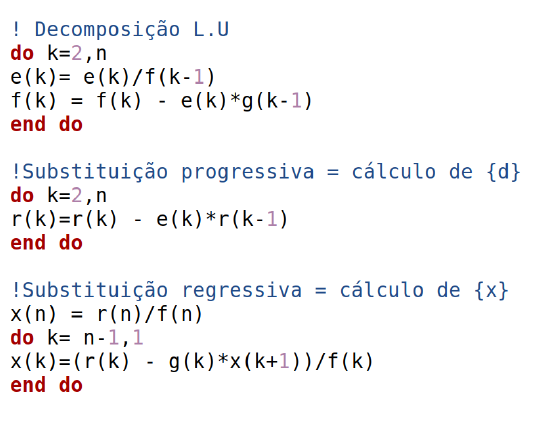
\includegraphics[width=0.8\textwidth]{img/algoritmo_thomas.png}
\caption{Pseudocódigo do Algoritmo de Thomas fornecido pelo professor.}
\end{figure}

Para o primeiro laço - \textit{!Documposição L.U}:

\begin{table}[H]
\centering
\begin{tabular}{|c|c|c|}
\hline
\textbf{Iteração} & \textbf{Valor de $e_k$} & \textbf{Valor de $f_k$} \\
\hline
fsrt &  & $f_1 = 2.04$ \\
scnd & $e_1 = -0.4902$ & $f_2 = 1.5498$ \\
thrd & $e_2 = -0.6452$ & $f_3 = 1.3948$ \\
frth & $e_3 = -0.717$ & $f_4 = 1.323$ \\
\hline
\end{tabular}
\caption{Valores de $e_k$ e $f_k$ durante as iterações do Algoritmo de Thomas.}
\label{tab:thomas_iterations}
\end{table}

\textit{!Substituição progressiva = cálculo de $\{d\}$}:

\begin{table}[H]
\centering
\begin{tabular}{|c|c|}
\hline
\textbf{Iteração} & \textbf{Valor de $r_k$} \\
\hline
fsrt & $r_1 = 40.8$ \\
scnd & $r_2 = 20.8$ \\
thrd & $r_3 = 14.2210$ \\
frth & $r_4 = 210.9961$ \\
\hline
\end{tabular}
\caption{Valores de $r_k$ durante as iterações do Algoritmo de Thomas.}
\label{tab:thomas_r_values}
\end{table}

\newpage
\textit{!Substituição regressiva = cálculo de \{x\}}:

\begin{table}[H]
\centering
\begin{tabular}{|c|c|}
\hline
\textbf{Iteração} & \textbf{Valor de $x_k$} \\
\hline
fsrt & $x_1 = 65.9698$ \\
scnd & $x_2 = 93.7785$ \\
thrd & $x_3 = 124.5382$ \\
frth & $x_4 = 159.4795$ \\
\hline
\end{tabular}
\caption{Valores de $x_k$ durante as iterações do Algoritmo de Thomas.}
\label{tab:thomas_x_values}
\end{table}

\paragraph{Comparação dos procedimentos}

A decomposição L.U. padrão exige um número significativamente maior de operações de ponto flutuante, dado que não explora a estrutura tridiagonal do sistema, realizando eliminações e atualizações em toda a matriz, totalizando aproximadamente \(\Theta(n^3)\) operações. Por outro lado, o Algoritmo de Thomas é otimizado para sistemas tridiagonais, reduzindo a complexidade para \(\Theta(n)\), com cerca de \(8n\) operações elementares. Assim, além de computacionalmente mais eficiente, o Algoritmo de Thomas apresentou resultados idênticos à decomposição L.U., confirmando sua confiabilidade e precisão para esse tipo de sistema. A equivalência dos vetores solução \{x\} valida ambos os métodos, mas a eficiência algorítmica do Thomas é claramente superior para sistemas dessa natureza.

\section{Enunciado 3 - Decomposição de Cholesky}
Invente um sistema linear se sua escolha no qual a matriz dos coeficientes seja uma matriz
quadrada, simétrica, de ordem 3. Você pode escolher os números que quiser para compor
a matriz dos coeficientes e o vetor {b}, desde que a matriz [A] seja simétrica. Em seguida,
aplique as relações de recorrência associdas `a decomposição de Cholesky e resolva o sistema
linear proposto.

\paragraph{Resolução} Consideremos a matriz simétrica e definida positiva:

\[
[A] = \begin{bmatrix}
4 & 2 & -2 \\
2 & 10 & -4 \\
-2 & -4 & 9
\end{bmatrix}, \quad
\{b\} = \begin{Bmatrix}
  2 \\
  6 \\
  5
\end{Bmatrix}
\]

Faremos \([L]\cdot[L]^{T}\), que segue a seguinte estrutura:

\[
[L] = \begin{bmatrix}
l_{11} & 0 & 0 \\
l_{21} & l_{22} & 0 \\
l_{31} & l_{32} & l_{33}
\end{bmatrix} \cdot
\begin{bmatrix}
l_{11} & l_{21} & l_{31} \\
0 & l_{22} & l_{32} \\
0 & 0 & l_{33}
\end{bmatrix} =
\begin{bmatrix}
  l_{11}^2 & l_{11}l_{21} & l_{11}l_{31} \\
  l_{11}l_{21} & l_{21}^2 + l_{22}^2 & l_{21}l_{31} + l_{22}l_{32} \\
  l_{11}l_{31} & l_{21}l_{31} + l_{22}l_{32} & l_{31}^2 + l_{32}^2 + l_{33}^2
\end{bmatrix}
\]

\subsection{Construção da matriz [L]}

Aplicamos o método clássico de Cholesky, onde $[A] = [L][L]^T$, com $[L]$ triangular inferior.

Para $l_{11}$:

\[
l_{11} = \sqrt{a_{11}} = \sqrt{4} = 2
\]

Para $l_{21}$:

\[
l_{21} = \frac{a_{12}}{l_{11}} = \frac{2}{2} = 1
\]

Para $l_{31}$:

\[
l_{31} = \frac{a_{13}}{l_{11}} = \frac{-2}{2} = -1
\]

Para $l_{22}$:

\[
l_{22} = \sqrt{a_{22} - l_{21}^2} = \sqrt{10 - 1} = \sqrt{9} = 3
\]

Para $l_{32}$:

\[
l_{32} = \frac{a_{23} - l_{31}l_{21}}{l_{22}} = \frac{-4 - (-1)(1)}{3} = -\frac{3}{3} = -1
\]

Para $l_{33}$:

\[
l_{33} = \sqrt{a_{33} - l_{31}^2 - l_{32}^2} = \sqrt{9 - 1 - 1} = \sqrt{7} = 2.6458
\]

\hspace{2cm}
\paragraph{Matriz [L] obtida}

\[
[L] = \begin{bmatrix}
2 & 0 & 0 \\
1 & 3 & 0 \\
-1 & -1 & 2.6458
\end{bmatrix}
\]

\subsection{Resolução do sistema}

Para resolver $[A]\{x\} = \{b\}$, aplicamos substituição progressiva em $[L]\{y\} = \{b\}$ e depois substituição regressiva em $[L]^T\{x\} = \{y\}$.

\[
[L] \cdot \{y\} = \{b\}
\]
\[
\begin{bmatrix}
2 & 0 & 0 \\
1 & 3 & 0 \\
-1 & -1 & 2.6458
\end{bmatrix} \cdot
\begin{Bmatrix}
y_1 \\
y_2 \\
y_3
\end{Bmatrix} =
\begin{Bmatrix}
2 \\
6 \\
5
\end{Bmatrix}
\]
\[
\{y\} = \begin{Bmatrix}
  1 \\
  1.6667 \\
  2.8977
\end{Bmatrix}
\]

Resolvendo \{x\} por substituição regressiva:

\[
[L]^T \cdot \{x\} = \{y\}
\]
\[
\begin{bmatrix}
2 & 1 & -1 \\
0 & 3 & -1 \\
0 & 0 & 2.6458
\end{bmatrix} \cdot
\begin{Bmatrix}
x_1 \\
x_2 \\
x_3
\end{Bmatrix} =
\begin{Bmatrix}
  1 \\
  1.6667 \\
  2.8977
\end{Bmatrix}
\]

\[
\{x\} = \begin{Bmatrix}
  0.5873 \\
  0.9206 \\
  1.0952
\end{Bmatrix}
\]

\newpage
\section{Enunciado 4 - Método de Gauss-Seidel com e sem relaxação}
Use o método de Gauss-Seidel ($a$) sem relaxamento e ($b$) com relaxamento (utilizando $\lambda = 1.2$)
para resolver o seguinte sistema de equações com um erro relativo de $5\%$. Se necessário,
reorganize as equações para garantir a convergência.

\[
\begin{cases}
2x_1 - 6x_2 - x_3 = -38 \\
- 3x_1 - x_2 + 7x_3 = -34 \\
-8x_1 + x_2 - 2x_3 = -20 \\
\end{cases}
\]

Considerando e reorganizando o sistema linear, teremos:

\[
\begin{cases}
-8x_1 + x_2 - 2x_3 = -20 \\
2x_1 - 6x_2 - x_3 = -38 \\
- 3x_1 - x_2 + 7x_3 = -34 \\
\end{cases}
\]

Isolando \(x\):

\[
\begin{cases}
x_1 = \frac{20 + x_2 -2x_3}{8} \\
x_2 = \frac{38 + 2x_1 - x_3}{6} \\
x_3 = \frac{-34 + 3x_1 + x_2}{7} \\
\end{cases}
\]


\subsection{Gauss-Seidel sem relaxação}

Partimos de uma aproximação inicial $\{x^{(0)}\} = \{0, 0, 0\}$.

Iterações até convergência ($\varepsilon < 5\%$):

\begin{table}[H]
  \centering
  \begin{tabular}{|c|c|c|c|c|}
    \hline
    \textbf{Variável} & \textbf{$k_1$} & \textbf{$k_2$} & \textbf{$k_3$} & \textbf{$k_4$} \\
    \hline
    $x_1$ & 2.5 & 4.0863 & 4.0047 & 3.9988 \\
    $x_2$ & 7.1667 & 8.1556 & 7.9917 & 7.9995 \\
    $x_3$ & -2.7619 & -1.9408 & -1.9992 & -2.0006 \\
    \hline
  \end{tabular}
  \caption{Iterações de Gauss-Seidel sem relaxação.}
  \label{tab:gs_s_relaxacao}
\end{table}

\subsection{Gauss-Seidel com relaxação}

Utilizamos fator de relaxação $\lambda = 1.2$:

Para cada $x_i^{(k)}$, ajustamos:

\[
x_i^{(k)} = x_i^{(k-1)} + \lambda\left(x_i^{*} - x_i^{(k-1)}\right)
\]

Iterações:

\begin{table}[H]
  \centering
  \resizebox{\textwidth}{!}{
  \begin{tabular}{|c|c|c|c|c|c|c|c|c|c|c|c|}
    \hline
    \textbf{Variável} & \textbf{$\lambda_1$} & \textbf{$k_2$} & \textbf{$\lambda_2$} & \textbf{$k_3$} & \textbf{$\lambda_3$} &  \textbf{$k_4$} & \textbf{$\lambda_4$} & \textbf{$k_5$} & \textbf{$\lambda_5$} & \textbf{$k_6$} & \textbf{$\lambda_6$} \\
    \hline
    $x_1$ & 3 & 4.4036 & 4.6843 & 3.8805 & 3.7198 & 4.0430 & 4.1077 & 3.9838 & 3.9590 & 4.0062 & 4.0156 \\
    $x_2$ & 8.6 & 8.4471 & 8.4166 & 7.7922 &7.6674 & 8.0923 & 8.1773 & 7.9608 & 7.9175 & 8.0162 & 8.0359 \\
    $x_3$ & -3.3143 & -1.6472 & -1.3138 & -2.1676 & -2.3384 & -1.9286 & -1.8466 & -2.0294 & -2.0659 & -1.9882 & 1.9726\\
    \hline
  \end{tabular}
  }
  \caption{Iterações de Gauss-Seidel com relaxação.}
  \label{tab:gs_c_relaxacao}
\end{table}

\subsection{Comparação}

A introdução da relaxação, com o fator \(\lambda=1.2\), não resultou em aceleração da convergência neste caso específico. As iterações foram conduzidas até que os erros relativos estivessem abaixo de 5\%. Observou-se que, sob essas condições, o método de Gauss-Seidel com relaxação exigiu um maior número de iterações em comparação à versão sem relaxação. Este comportamento evidencia que a escolha inadequada do fator de relaxação pode comprometer a eficiência do método, reforçando a necessidade de calibração criteriosa para sistemas diagonais dominantemente estritos.

\section{Conclusões}

Foram aplicadas quatro técnicas distintas de resolução de sistemas lineares. Destacou-se a precisão das decomposições L.U. e Cholesky, a eficiência do Algoritmo de Thomas para sistemas tridiagonais, e a rapidez de convergência do método de Gauss-Seidel. A análise reforça a importância de selecionar o método adequado conforme a estrutura do sistema linear.

\end{document}
